\documentclass[a4paper]{article}

\usepackage{fullpage} % Package to use full page
\usepackage{parskip} % Package to tweak paragraph skipping
\usepackage{tikz} % Package for drawing
\usepackage{amsmath}
\usepackage{hyperref}
\usepackage[utf8]{inputenc}
\usepackage{graphicx}
\usepackage{enumitem}
\usepackage{booktabs}
\usepackage{lmodern}
\usepackage[MeX]{polski}
\usepackage[T1]{fontenc}
\usepackage{float}
\usepackage{subfiles}

\title{Notatki z kursu Inżynieria Oprogramowania}
\author{Małgorzata Dymek}
\date{2018/19, semestr letni}

\graphicspath{{graphics/}}

\begin{document}
    \maketitle

    \section{Podstawowe pojęcia}
    \begin{table}[H]
        \begin{center}
            \begin{tabular}{  p{6cm} p{10cm}  }

                \textbf{Scenariusz przypadku użycia} - wyspecyfikowana \underline{sekwencja zdarzeń} między użytkownikiem a systemem.
                &
                \begin{itemize}
                    \item Zdefiniowane w pierwszej kolejności.
                    \item Wyróżnia się jeden \textbf{główny scenariusz sukcesu}.
                    \item Może zawierać warunki wstępne, gwarancje lub wyzwalacze.
                    \item W agile development używa się \underline{skróconej wersji scenariusza} odpowiadającej
                    na pytania:kto, co, dlaczego.
                \end{itemize}
                \\

                \cmidrule(r){1-1}\cmidrule(l){2-2}

                \textbf{Przypadek użycia} - \underline{zbiór powiązanych ze sobą scenariuszy} opisujących użycie systemu przez aktorów.
                &
                Opisujemy je tekstowo, poprzez user stories lub diagramy.
                \begin{itemize}
                    \item reprezentuje \textbf{funkcjonalne wymaganie} systemu;
                    \item pewna historia; opisuje akcje systemu z punktu widzenia użytkownika;
                    \item specyfikuje jeden aspekt zachowania bez wchodzenia w strukturę systemu;
                    \item jest zorientowany na osiągnięcie celu użytkownika;
                \end{itemize}
                \\

            \end{tabular}
        \end{center}
    \end{table}

    \section {UML}
    \begin{figure}[H]
        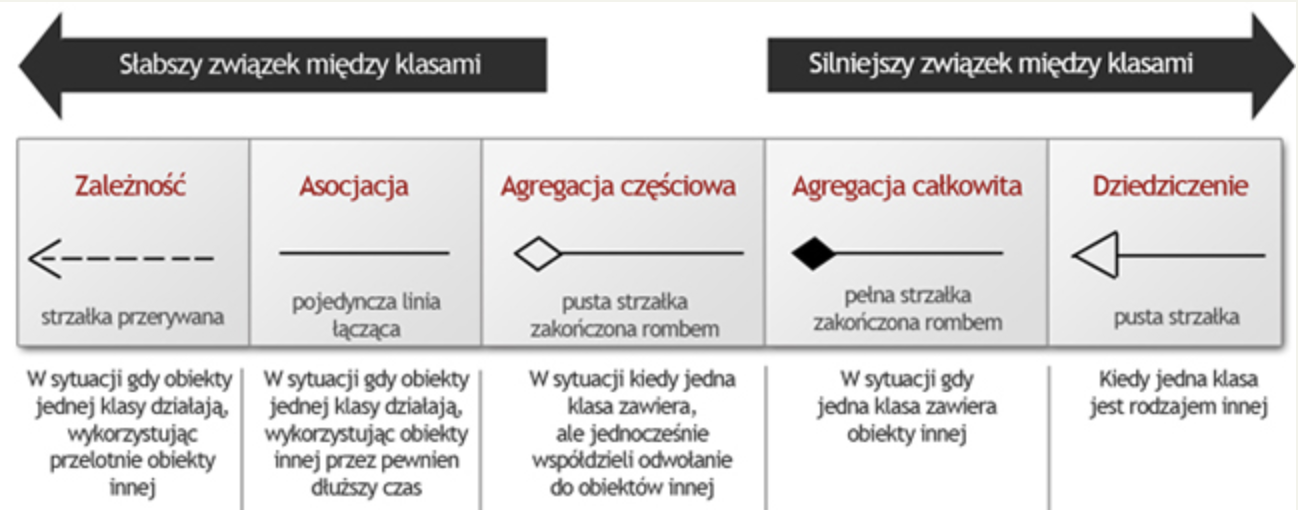
\includegraphics[width=\linewidth]{uml_zwiazki.png}
    \end{figure}

    \section{Procesy wytwarzania oprogramowania}
    \textbf{Cztery fundamentalne działania }wspólne dla wszystkich procesów:
    \begin{itemize}
        \item \textbf{Specyfikowanie} oprogramowania
        \item \textbf{Tworzenie} oprogramowania
        \item \textbf{Walidacja} oprogramowania
        \item \textbf{Ewolucja} oprogramowania
    \end{itemize}


    \subsection{Modele procesu wytwarzania oprogramowania}
    \begin{table}[H]
        \begin{center}
            \begin{tabular}{ p{4cm} p{11cm}  }

                \textbf{Model kaskadowy}
                &
                \begin{itemize}
                    \item \textbf{wyizolowane etapy}: Planowanie, Analiza, Projekt, Implementacja, Testowanie, Pielęgnacja,
                    \item etapy podzielone na dwie części: \underline{twórczą} i \underline{weryfikacji},
                    \item bardzo wysoki koszt błędów
                    popełnionych we wstępnych etapach, adaptowanie zmian bardzo kosztowne,
                    \item powinien bvyć używany tylko jeśli wymagania są jasne i zrozumiałe,
                    \item marginalizacja roli klienta w procesie wytwarzania oprogramowania.
                \end{itemize}
                \\

                \cmidrule(r){1-1}\cmidrule(l){2-2}

                \textbf{Model V}
                &
                \begin{itemize}
                    \item wymagania klienta - testy akceptacyjne
                    \item wymagania systemowe - testy systemowe
                    \item ogólny design - testy integracyjne
                    \item szczegółowy design - testy modułowe
                \end{itemize}
                \\

                \cmidrule(r){1-1}\cmidrule(l){2-2}

                \textbf{Model Ewolucyjny}
                &
                \begin{itemize}
                    \item równolegle przeprowadzana specyfikacja, rozwój systemu i weryfikacja
                    \item pozwala później określić wymagania do projektowanego systemu,
                    \item prototyp: pomaga kształcić przyszłego użytkownika, podnosi koszty
                    w krótszej perspektywie, ale w dłuższej może je obniżać, zwykle jest wyrzucany.
                \end{itemize}
                \\

                \cmidrule(r){1-1}\cmidrule(l){2-2}

                \textbf{Model iteracyjny}
                &
                \begin{itemize}
                    \item planowanie, projektowanie, testowanie, prototypowanie,
                    \item całościowe myślenie o produkcie,
                    \item pozwala na wczesne wykrywanie błędów, łatwość wprowadzania zmian,
                    \item wymogi klienta dotyczące harmonogramu mogą utrudnić korzystanie z tego
                    modelu,
                    \item problemy z oszacowaniem ryzyka.
                \end{itemize}
                \\

                \cmidrule(r){1-1}\cmidrule(l){2-2}

                \textbf{Model spiralny}
                &
                \begin{itemize}
                    \item planowanie, analiza, konstrukcja, weryfikacja,
                    \item ciągłe monitorowanie i pomiar zmian,
                    \item zmiany poddawane są review użytkownika,
                    \item próba minimalizacji ryzyka niepowodzenia.
                \end{itemize}
                \\

            \end{tabular}
        \end{center}
    \end{table}

    \section{Standardy jakości}

    Odpowiedź na syndrom \textbf{LOOP} - \textbf{L}ate, \textbf{O}ver budget, \textbf{O}vertime, \textbf{P}oor quality.

    \begin{table}[H]
        \begin{center}
            \begin{tabular}{ p{7cm} | p{9cm}  }

                \textbf{CMM - Capability Maturity Model}

                \textbf{Ocenia proces wytwórczy} w skali pięciostopniowej - od \textbf{chaotycznego} do \textbf{ścisłego}.
                &
                \begin{itemize}
                    \item Poziomy dojrzałości
                    \begin{itemize}
                        \item Poziom 1 - Wstępny.
                        \item Poziom 2 - Powtarzalny.
                        \item Poziom 3 - Zdefiniowany.
                        \item Poziom 4 - Zarządzany.
                        \item Poziom 5 - Optymalizujący.
                    \end{itemize}

                    \item Kluczowe obszary procesowe - podzielone na pięć cech - podzielone na kluczowe praktyki.
                \end{itemize}
                \\

                \cmidrule(r){1-1}\cmidrule(l){2-2}

                \textbf{ISO 9000}

                Wymaga \textbf{udokumentowania wszystkich procedur} związanych z wytwarzaniem oprogramowania.
                &
                \begin{itemize}
                    \item Odpowiedzialność kierownictwa
                    \item Zarządzanie zasobami
                    \item Realizacja wyrobu
                    \item Pomiary, analiza i doskonalenie
                    \item Ciągłe doskonalenie systemu zarządzania jakością
                \end{itemize}
                \\
            \end{tabular}
        \end{center}
    \end{table}


    \section{Zwinne procesy wytwarzania oprogramowania}

    \subsection{Programowanie ekstremalne - XP}
    \begin{itemize}
        \item brak fazy projektowania i dokumentacji,
        \item krótka perspektywa planowania,
        \item silne założenie, że klient pracuje cały czas z zespołem.
    \end{itemize}



    \begin{itemize}
        \item \textbf{Struktura zespołu} - role podstawowe (programiści, klient) i pomocnicze
        (tester, coach, tracker).

        \item \textbf{User Stories} - pisują \textbf{funkcje systemu} z punktu widzenia użytkownika,

        \item \textbf{Gra planistyczna} - pisanie (klient), oszacowanie (informatycy) i dzielenie
        (klient) user story,

        \item \textbf{Zapewnianie jakości} - prostota, TTD, automatyczne testowanie, refaktoryzacja.

        \item \textbf{Testy akceptacyjne} - od klienta, najlepiej automatycznie.

        \item \textbf{Programowanie parami} - wspólny standard kodowania, częste zmiany par, system
        kontroli wersji.
    \end{itemize}

    \begin{table}[H]
        \begin{center}
            \begin{tabular}{ p{2cm} p{14cm}}
                \textbf{Wartości}
                &
                \begin{itemize}
                    \item \textbf{Komunikacja} - przede wszystkim werbalna.
                    \item \textbf{Prostota} - rozpoczynamy od najprostszego rozwiązania.
                    \item \textbf{Sprzężenie zwrotne} - obejmuje kilka aspektów (system, klient, zespół).
                    \item \textbf{Odwaga} - potrzebna by: od razu produkować kod; refaktoryzować; wyrzucić zbędny kod.
                    \item \textbf{Szacunek} - do pracy i czasu innych; między członkami zespołu.
                \end{itemize}
            \end{tabular}
        \end{center}
    \end{table}

    \subsection{SCRUM}

    \begin{table}[H]
        \begin{center}
            \begin{tabular}{ p{2.5cm} p{13.5cm}}
                \textbf{Trzy filary}
                &
                \begin{itemize}
                    \item \textbf{Adaptacja} - powinna być \underline{ciągła}.
                    \item \textbf{Przejrzystość} - \underline{istotne aspekty} procesu
                    muszą być \underline{widoczne} dla osób odpowiedzialnych.
                    \item \textbf{Inspekcja} – poddawane \underline{regularnej} inspekcji.
                \end{itemize}
                \\
                % \cmidrule(r){1-2}

                \textbf{Role}
                &
                \begin{itemize}
                    \item \textbf{Właściciel Produktu} - odpowiedzialny za pracę ZD, zarządza RP.
                    \item \textbf{Zespoł deweloperski} - samoorganizujący się, wielofunkcyjny, zarządza RS.
                    \item \textbf{Scrum Master}.
                \end{itemize}
                \\


                \textbf{Artefakty}
                &
                \begin{itemize}
                    \item \textbf{Rejestr Produktu} - uporządkowana lista wszystkiego, co może być potrzebne
                    w produkcie.
                    \item \textbf{Rejestr Sprintu} - podzbió RP wybrany do Sprintu rozszerzony o plan
                    dostarczenia Przyrostu produktu.
                    \item \textbf{Monitorowanie postępów Sprintu} - możliwe w każdym momencie Sprintu.
                    \item \textbf{Przyrost} - suma wszystkich elementów RP zakończonych podczas wszystkich sprintów.
                    \item \textbf{Definicja Ukończenia}
                \end{itemize}
                \\

                \textbf{Zdarzenia}
                &
                \begin{itemize}
                    \item \textbf{Sprint} – stały czas, niezmienny cel, niezmienny skład ZD.
                    \item \textbf{Przerwanie Sprintu} - tylko przez WP, przy deaktualizacji celu.
                    \item \textbf{Planowanie Sprintu} - 8h/mies, wyznaczenie celu, projektu systemu i planu prac.
                    \item \textbf{Codzienny Scrum} - 15 min/d.
                    \item \textbf{Przegląd Sprintu} - 4h na zakończenie Sprintu.
                    \item \textbf{Retrospektywa Sprintu} - inspekcja i opracowanie planu usprawnień.
                \end{itemize}
            \end{tabular}
        \end{center}
    \end{table}


    \subsection{AGILE PM (DSDM Atern)}

    \begin{table}[H]
        \begin{center}
            \begin{tabular}{ p{2.5cm} p{13.5cm}}
                \textbf{Role}
                &
                \begin{itemize}
                    \item \textbf{Business Sponsor} - najwyższy rangą w projekcie; zapewnia finansowanie i zasoby.
                    \item \textbf{Business visionary} - definiuje wizję projektu i komunikuje ją.
                    \item \textbf{Project manager} - monitoruje postęp projektu, wysoko poziomowe planowanie.
                    \item \textbf{Technical coordinator} - definiuje środowisko pracy, pilnuje standardów, zajmuje się wymaganiami niefunkcjonalnymi.
                    \item \textbf{Team Leader}.
                    \item \textbf{Business Ambassador} - rola biznesowa w zespole deweloperskim, tworzy dokumentacje użytkownika.
                    \item \textbf{Business Analyst} - komunikacja między biznesem a zespołem deweloperskim.
                    \item \textbf{Solution Developer} - skupiony na dostarczeniu rozwiązania.
                    \item \textbf{Solution Tester} - definiuje scenariusze testowe, test casy.
                \end{itemize}
                \\

                \textbf{Fazy projektu}
                &
                \begin{itemize}
                    \item \textbf{Pre-project} - identyfikacja BS i BV; zakresu, planu i zasobów na Feasibility.
                    \item \textbf{Feasibility} - wykonalność, zyskowność, czasowość, kosztowość.
                    \item \textbf{Foundation} - wysoko poziomowe wymagania.
                    \item \textbf{Exploration} - uszczegóławianie wymagań; iteracyjnie działające możliwe rozwiązanie.
                    \item \textbf{Engineering} - rozwijanie rozwiązania z fazy Exploration.
                    \item \textbf{Deployment} - potwierdzenie wydajności rozwiązania, dostarczenie rozwiązania i dokumentacji.
                \end{itemize}
                \\
            \end{tabular}
        \end{center}
    \end{table}

    \begin{table}[H]
        \begin{center}
            \begin{tabular}{ p{2.5cm} p{13.5cm}}
                \textbf{Produkty}
                &
                \begin{itemize}
                    \item Levels of priority - \textbf{MoSCoW}: \textbf{M}ust Have,
                    \textbf{S}hould Have, \textbf{C}ould Have, \textbf{W}on’t Have this time
                \end{itemize}
                \\

                \textbf{TIMEBOX}
                &
                \begin{itemize}
                    \item \textbf{Kick-off} – krótka sesja, która ma pomoc zrozumieniu celu timeboxa,
                    \item \textbf{Investigation} – szczegóły wszystkich produktów, które mamy wykonać,
                    \item \textbf{Refinement} – kodowanie i testowanie,
                    \item \textbf{Consolidation} – spinanie całości.
                \end{itemize}
                \\

                \textbf{Iterative development}
                &
                \begin{itemize}
                    \item \textbf{Identify}: zespół definiuje cel
                    \item \textbf{Plan}: kto powinien zrobić co
                    \item \textbf{Evolve}: wykonywanie
                    zaplanowanych czynności
                    \item \textbf{Review}: sprawdzanie rezultatów
                \end{itemize}
            \end{tabular}
        \end{center}
    \end{table}


    \subsection{AUP - Agile Unified Process}

    \begin{itemize}
        \item stosuje zwinne techniki takie jak TDD, refactoring,
        \item \textbf{seryjny w dużej skali, iteracyjny w małej}.
    \end{itemize}

    \textbf{Zasady AUP}
    \begin{itemize}
        \item twój zespół wie, co robi;
        \item prostota;
        \item zwinność;
        \item skupienie się na istotnych aktywnościach;
        \item niezależność od narzędzi;
        \item możliwość adaptacji.
    \end{itemize}



    \subsection{KANBAN}


    \begin{itemize}
        \item \textbf{ciągły przepływ produktu przez system produkcyjny}.
        \item \textbf{system pull} sterowany
        jest przez \textbf{składane przez odbiorcę zamówienie}, a nie ogólny, arbitralny plan produkcji.
        \item odnosi się do \textbf{etapowości procesu wytwarzania
        oprogramowania}, przynajmniej trzy stany pracy — do zrobienia, w trakcie, gotowe.
        \item możliwość specjalizacji w zespołach
        \item nie identyfikuje "Ukończenia"
    \end{itemize}


    \textbf{Sześć reguł kanbana}:
    \begin{itemize}
        \item odbiorca przetwarza dokładnie tyle elementów, ile opisane jest na karcie kanban;
        \item dostawca wytwarza dokładnie tyle elementów, ile opisane jest na karcie kanban;
        \item żaden element nie jest wytwarzany lub przekazywany pomiędzy stanowiskami bez karty kanban;
        \item karta kanban musi towarzyszyć każdemu elementowi czy półproduktowi przetwarzanemu w ramach systemu;
        \item elementy wadliwe lub występujące w niewłaściwych ilościach, nigdy nie są przekazywane w dół procesu;
        \item limity obowiązujące na każdym z etapów (fizyczna ilość kart kanban) są stopniowo obniżane aby redukować zapasy i
        odkrywać nieefektywności procesów produkcji, dążąc do ich doskonalenia.
        \item postęp prac monitorowany na tablicy kanban oraz poprzez analizę średnich czasów wykonania\\
    \end{itemize}


    \subsection{SCRUM-BAN}
    \begin{itemize}
        \item board
        \item tylko daily scrum, płynna praca
        \item zespoły mogą być specjalizowane, role jak potrzeba
        \item WIP kontrolowane przez workflow, zmiany dodawane do TODO board na bieżąco
        \item product backlog tylko w kartkach czasowych
    \end{itemize}


    \section{Wymagania}
    \textbf{Klasyfikacja wymagań - FURPS} - \textbf{F}unctionality, \textbf{U}sability, \textbf{R}eliability,
    \textbf{P}erformance, \textbf{S}ecurity.


    \begin{itemize}
        \item \textbf{Funkcjonalne} - czynność, zadanie, „System powinien\dots”.
        \item \textbf{Pozafunkcjonalne} - technikalia mierzone metrykami.
        \begin{itemize}
            \item \textbf{Niezawodność} - odporność na błędy, dojrzałość.
            \item \textbf{Wydajność}.
            \item \textbf{Użyteczność} - łatwość zrozumienia i nauki, operatywność.
            \item \textbf{Łatwość konserwacji} - łatwość analizy, wprowadzania zmian, testowania; stabilność.
            \item \textbf{Przenośność} - łatwość adaptacji, instalacji.
        \end{itemize}
    \end{itemize}

    Cecha \textbf{INVEST}: Independent, Negotiable, Valuable, Estimable, Small, Testable.

    \textbf{Analiza wymagań/analiza obiektowa}
    \begin{itemize}
        \item Celem jest stworzenie modelu systemu, zwanego \textbf{modelem analitycznym}.
        \item Wysiłek uczestników projektu skupia się na strukturalizowaniu i formalizowaniu zabranych
        wcześniej wymagań.

        \item \textbf{Model analityczny} – system z perspektywy użytkownika.
        \item \textbf{Analityczny model obiektowy}.
        \item \textbf{Model dynamiczny} - koncentruje się na zachowaniu systemu.
        \item \textbf{Obiekty encji} – reprezentują trwałą informację potwarzaną przez system.
        \item \textbf{Obiekty brzegowe} – odzwierciedlają interakcje między aktorami a systemem.
        \item \textbf{Obiekty sterujące} – odpowiedzialne są za realizację przypadków użycia.
        \item \textbf{Relacja dziedziczenia} umożliwia hierarchiczne organizowanie koncepcji.
        \item \textbf{Generalizowanie} - aktywność identyfikowania abstrakcyjnych koncepcji na podstawie przykładów i konkretyzacji.
        \item \textbf{Specjalizowanie} - aktywność odwrotna, czyli identyfikowanie koncepcji bardziej specyficznych na podstawie koncepcji wysokopoziomowej.
    \end{itemize}


    \section{Projektowanie systemu}
    \begin{itemize}
        \item rozpoznawanie celów projektowych,
        \item projektowanie wstępnych dekompozycji,
        \item doskonalenie dekompozycji stosownie do celów projektowych.
    \end{itemize}

    \subsection{Podstawowe pojęcia i koncepcje.}
    \begin{itemize}
        \item \textbf{Podsystem} - wymienna część systemu, posiadającą dobrze zdefiniowane interfejsy i
        hermetyzującą stan oraz zachowanie składających się na nią klas.
        \item Dwa główne typy komponentów: \textbf{logiczny i fizyczny}.
        \item \textbf{Usługa} jest zbiorem powiązanych operacji podporządkowanych realizacji wspólnego
        celu.
        \item \textbf{Sprzężeniem} w zbiorze podsystemów nazywamy stopień ich \textbf{wzajemnego uzależnienia}. (MINIMALIZACJA)
        \item \textbf{Spoistość} podsystemu jest miara \textbf{uzależnienia jego własnych klas}. (MAKSYMALIZACJA)
        \item \textbf{Warstwa} - zgrupowanie podsystemów oferujących powiązane usługi.
        \item Efektem \textbf{dekompozycji hierarchicznej} jest uporządkowany zbiór warstw.
        \item \textbf{Architektury warstwowa}: otwarta i zamknięta (np ISO/OSI, TCP/IP).
    \end{itemize}


    \subsection{Wzorce architektoniczne - poziom integracji komponentów}


    \begin{table}[H]
        \begin{center}
            \begin{tabular}{ p{.3\textwidth} p{.5\textwidth} p{.2\textwidth}}
                \toprule
                Model & Opis & Zastosowanie\\
                \toprule

                MVC: Model-Widok-Kontroler
                &
                Model zawiera korowa funkcjonalność. Widoki wyświetlają funkcjonalności. Kontroler obsługuje żądanie użytkownika. Kontroler z widokami tworzą UI aplikacji.
                &
                Smalltalk, Java/Swing.\\

                \cmidrule(l){1-3}

                PAC: Prezentacja-Abstrakcja-Kontrola
                &
                Hierarchie kooperujących agentów,podzielonych na trzy komponenty: prezentacji, abstrakcji kontroli.
                &
                Network Trafic Management (gathering traffic datha, displaying various user-configurable
                views of the whole network).\\

                \cmidrule(l){1-3}

                Architektura filtry i potoki
                &
                Pozwala na uporządkowanie systemu, który przetwarza strumienie danych. Każdy krok przetwarzania jest zamknięty w filtrze.
                Dane są przesyłane za pomocą potoków. Każdy z podsystemów realizuje przetwarzanie danych otrzymanych od innych podsystemów.
                &
                Unix, WEB, Servlet, Numerical Analysis (filters and data extractions).\\

                \cmidrule(l){1-3}

                Tablica (blackboard)
                &
                Użyteczna w systemach, gdzie nie są znane deterministyczne rozwiązania danego problemu. W przypadku tablicy kilka wyspecjalizowanych
                systemów łączy swoja wiedze w taki sposób, żeby stworzyć częściowe lub przybliżone rozwiązanie problemu.
                &
                Working memory, repository data.\\

                \cmidrule(l){1-3}

                Broker
                &
                Pozwala na uporządkowanie rozproszonych systemów podzielonych na komponenty współpracujące ze sobą za pomocą zdalnego wywoływania
                serwisu. Komponent brokera odpowiedzialny jest za koordynację komunikacji.
                & \\

                \cmidrule(l){1-3}

                Reflection &
                Dostarcza mechanizm pozwalający na dynamiczną zmianę zachowania i struktury systemu.
                & WWW.\\

                \toprule
                \multicolumn{3}{c}{Sieciowe}\\
                \toprule

                Architektura klient-serwer
                &
                Podział systemu na dostawce usług (serwer) oraz ich odbiorców (klientów).
                & \\

                \cmidrule(l){1-3}

                Architektura peer-to-peer
                &
                Każdy z podsystemów może spełniać obie funkcje (klient/serwer).
                & \\

                \bottomrule
            \end{tabular}
        \end{center}
    \end{table}

    \begin{itemize}
        \item Patterns do not lead to direct code reuse.
        \item Individual Patterns are deceptively simple.
        \item Composition of different patterns can be very complex.
        \item Teams may suffer from pattern overload.
        \item Patterns are validated by experience and discussion
        rather than by automated testing.
        \item Integrating patterns into a software development
        process is a human-intensive activity.
    \end{itemize}



    \section{Projektowanie obiektów}
    \begin{itemize}
        \item wykorzystanie gotowych rozwiązań, którymi są zarówno
        gotowe produkty (komponenty) jak i wzorce projektowe;
        \item specyfikowanie usług;
        \item restrukturyzacja modelu obiektowego;
        \item optymalizacja modelu obiektowego;
    \end{itemize}


    Koncepcje wielokrotnego wykorzystywania gotowych rozwiązań:
    \begin{itemize}
        \item \textbf{obiekty aplikacyjne} - reprezentują koncepcje problemowe związane z tworzonym systemem.
        \item \textbf{obiekty realizacyjne} - reprezentują komponenty nie mające odpowiedników w
        dziedzinie aplikacyjnej, na przykład bazy danych czy obiekty interfejsu użytkownika.
        \item \textbf{dziedziczenie implementacyjne} - ma miejsce jeśli sięgamy po dziedziczenie z zamiarem wykorzystania
        gotowego kodu, mimo różnic koncepcyjnych pomiędzy powiązanymi klasami.
        \item \textbf{dziedziczenie specyfikacyjne} - ma odzwierciedlenie w taksonomii klas (reprezentuje podtypowanie).
        \item \textbf{delegowanie implementacji} - zamiast implementować set jako nadpisywanie metod hashtable, implementujemy go jako set korzystajacy z instancji hashtable z własnymi metodami.
        Rozwiązuje problemy dziedziczenia implementacyjnego: rozszerzalność, podtypowanie.
        \item \textbf{zasada zastępowania Liskov} - \textit{'Jeśli obiekt klasy S może stać się substytutem obiektu klasy T w
        dowolnym miejscu kodu, w którym oczekiwany jest obiekt klasy T, to klasa S jest podtypem klasy T.'}
        \item \textbf{wzorce projektowe} (obiektowe);
    \end{itemize}



    \subsection{Wzorce projektowe - poziom interakcji między klasami}
    \textbf{Wzorzec opisuje problem, który powtarza się wielokrotnie w danym środowisku, oraz podaje istotę
    jego rozwiązania.}

    \begin{itemize}
        \item Czy typowe problemy można rozwiązać w powtarzalny sposób?
        \item Czy te problemy można przedstawić w sposób abstrakcyjny, tak aby były pomocne
        w tworzeniu rozwiązań w róznych konkretnych kontekstach?
    \end{itemize}

    \begin{itemize}
        \item \textbf{Wzorce kreacyjne}
        \begin{itemize}
            \item abstrakcyjne metody tworzenia obiektów,
            \item uniezależnienie systemu od sposobu tworzenia obiektów.
        \end{itemize}
        \item \textbf{Wzorce strukturalne}
        \begin{itemize}
            \item sposób wiązania obiektów w struktury,
            \item właściwe wykorzystanie dziedziczenia i kompozycji.
        \end{itemize}
        \item \textbf{Wzorce behawioralne}
        \begin{itemize}
            \item algorytmy i przydział odpowiedzialności,
            \item opis przepływu kontroli i interakcji.
        \end{itemize}
    \end{itemize}

    \subsection{Koncepcje specyfikowania interfejsów}
    \begin{itemize}
        \item implementator (realize class), ekstender (refine class) i użytkownik (use class) klasy,
        \item typy, sygnatury (wektory/krotki typów parametrów i typu wyniku) i widzialność (public, private, protected, packet),
        \item kontrakty: niezmienniki, warunki wstępne i warunki końcowe,
        \item język OCL (Object Constraint Language) – ograniczenia, zbiory, wielozbiory i ciągi; kwantyfikatory.
    \end{itemize}

    \subsection{Aktywności specyfikowania interfejsów}
    \begin{itemize}
        \item identyfikowanie brakujących atrybutów i operacji;
        \item definiowanie widzialności i sygnatur;
        \item specyfikowanie kontraktów;
        \item dziedziczenie kontraktów;
    \end{itemize}



    \subsection{SOLID}

    \begin{itemize}
        \item \textbf{Single responsibility principle}
        \item \textbf{Open/closed principle}
        \item \textbf{Liskov substitution principle}
        \item \textbf{Interface segregation principle}
        \item \textbf{Dependency inversion principle}
    \end{itemize}


    \begin{table}[H]
        \begin{center}
            \begin{tabular}{  p{3cm} p{12cm}  }
                \toprule
                \multicolumn{2}{c}{Wzorce kreacyjne}\\
                \toprule

                \textbf{Singleton}
                &
                \begin{itemize}
                    \item Zapewnienie, że \textbf{klasa posiada jedną instancję} wewnątrz całej aplikacji
                    \item Stworzenie punktu dostępowego do tej instancji
                \end{itemize}
                \\

                \cmidrule(r){1-1}\cmidrule(l){2-2}
                \textbf{Factory method}
                &
                \begin{itemize}
                    \item Zdefiniowanie \textbf{interfejsu do tworzenia obiektów}
                    \item Umożliwienie przekazania odpowiedzialności za tworzenie obiektów do podklas
                    \item Umożliwienie wyboru klasy i konstruktora użytego do utworzenia obiektu
                \end{itemize}
                \\

                \cmidrule(r){1-1}\cmidrule(l){2-2}
                \textbf{Builder}
                &
                \begin{itemize}
                    \item \textbf{Odseparowanie sposobu reprezentacji i metody konstrukcji} złożonych struktur obiektowych
                    \item Wykorzystanie jednego mechanizmu konstrukcyjnego do tworzenia struktur o różnej reprezentacji
                \end{itemize}\\

                \bottomrule

            \end{tabular}
        \end{center}
    \end{table}

    \begin{table}[H]
        \begin{center}
            \begin{tabular}{  p{3cm} p{12cm}  }
                \toprule
                \multicolumn{2}{c}{Wybrane wzorce strukturalne}\\
                \toprule

                \textbf{Adapter}
                &
                \begin{itemize}
                    \item Umożliwia \textbf{współpracę obiektów o niezgodnych typach}
                    \item Tłumaczy protokoły obiektowe
                \end{itemize}
                \\

                \cmidrule(r){1-1}\cmidrule(l){2-2}

                \textbf{Proxy}
                &
                \begin{itemize}
                    \item Dostarcza \textbf{zamiennik obiektu} w celu jego kontroli i ochrony
                    \item Przezroczyste odsuniecie inicjalizacji obiektu w czasie
                \end{itemize}
                \\

                \cmidrule(r){1-1}\cmidrule(l){2-2}
                \textbf{Fasada}
                &
                \begin{itemize}
                    \item Dostarczenie \textbf{jednorodnego interfejsu wyższego poziomu} do zbioru różnych interfejsów w systemie
                    \item Ukrycie złożoności podsystemów przed klientem
                \end{itemize}
                \\
                \bottomrule

            \end{tabular}
        \end{center}
    \end{table}

    \begin{table}[H]
        \begin{center}
            \begin{tabular}{  p{3cm} p{12cm}  }
                \toprule
                \multicolumn{2}{c}{Wybrane wzorce behawioralne}\\
                \toprule

                \textbf{Obserwator}
                &
                \begin{itemize}
                    \item Tworzy \textbf{zależność typu jeden-wiele} pomiędzy obiektami
                    \item \textbf{Informacja o zmianie} stanu wyróżnionego obiektu jest \textbf{przekazywana wszystkim pozostałym obiektom}
                \end{itemize}
                \\

                \cmidrule(r){1-1}\cmidrule(l){2-2}
                \textbf{Command}
                &
                \begin{itemize}
                    \item \textbf{Hermetyzacja poleceń} do wykonania w postaci obiektów
                    \item Umożliwienie \textbf{parametryzacji klientów} obiektami poleceń
                    \item Wsparcie dla \textbf{poleceń odwracalnych}
                \end{itemize}
                \\

                \cmidrule(r){1-1}\cmidrule(l){2-2}

                \textbf{Chain of responsibility}
                &
                \begin{itemize}
                    \item \textbf{Usunięcie powiązania pomiędzy nadawcą i odbiorcą} żądania
                    \item Umożliwienie wielu obiektom obsługi żądania
                \end{itemize}
                \\

                \cmidrule(r){1-1}\cmidrule(l){2-2}

                \textbf{Iterator}
                &
                \begin{itemize}
                    \item Umożliwienie \textbf{sekwencyjnego dostępu} do elementów kolekcji bez ujawniania jej wewnętrznej implementacji
                \end{itemize}
                \\
                \bottomrule
            \end{tabular}
        \end{center}
    \end{table}


    \subsection{Implementacja wzorców projektowych}

    \textbf{Transformacja}
    \begin{itemize}
        \item powinna dotyczyć tylko jednego, ściśle określonego kryterium,
        \item musi mieć charakter lokalny, powinna być izolowana od innych zmian,
        \item musi być poddana weryfikacji.
    \end{itemize}

    \begin{table}[H]
        \begin{center}
            \begin{tabular}{ p{8cm} p{8cm} }
                \item \textbf{Transformacja modelu}
                \begin{itemize}
                    \item ograniczona jest do samego modelu
                    \item celem jest uproszczenie lub zoptymalizowanie istniejącego modelu
                \end{itemize}
                &
                \item \textbf{Inżynieria postępująca}
                \begin{itemize}
                    \item tworzenie szablonów kodu źródłowego odpowiadającego modelowi obiektowemu
                \end{itemize}\\
            \end{tabular}
        \end{center}
    \end{table}

    \textbf{Najczęściej wykonywane} aktywności (transformacje):
    \begin{itemize}
        \item \textbf{optymalizowanie modelu} obiektowego,
        \item odwzorowywanie \textbf{skojarzeń w kolekcje},
        \item odwzorowywanie \textbf{kontraktów w wyjątki},
        \item odwzorowywanie modelu obiektowego w \textbf{schematy bazy danych}.
    \end{itemize}


    \subsubsection{Paradygmat programowania}
    \begin{itemize}
        \item wzorzec, \textbf{najogólniejszy model}, jako wzorcowy przykład,
        \item \textbf{zbiór pojęć} i teorii tworzących \textbf{podstawy} danej nauki.
    \end{itemize}

    \begin{table}[H]
        \begin{center}
            \begin{tabular}{  p{3cm} p{12cm}  }
                \textbf{Abstrakcja} &
                System jako układ obiektów, które mogą:
                \begin{itemize}
                    \item opisywać i zmieniać swój stan,
                    \item komunikować się z innymi obiektami w systemie,
                    \item wykonywać pewne czynności na rzecz innych obiektów bez ujawniania, w jaki sposób zaimplementowano
                    dane cechy.
                \end{itemize}\\


                \textbf{Enkapsulacja}
                &
                \begin{itemize}
                    \item ukrywanie szczegółów implementacji,
                    \item obiekt nie może zmieniać stanu wewnętrznego innych obiektów w nieoczekiwany sposób,
                    \item tylko wewnętrzne metody obiektu są uprawnione do zmiany jego stanu,
                    \item każdy typ obiektu dostarcza innym obiektom swój "interfejs"
                \end{itemize}\\


                \textbf{Polimorfizm}
                &
                \begin{itemize}
                    \item wykazywanie różnych form działania w zależności od typu obiektu,
                    \item referencje i kolekcje obiektów mogą dotyczyć obiektów różnego typu
                \end{itemize}\\


                \textbf{Dziedziczenie}
                &
                \begin{itemize}
                    \item porządkuje i wspomaga polimorfizm i enkapsulację,
                    \item umożliwia definiowanie i tworzenie specjalizowanych obiektów,
                \end{itemize}
            \end{tabular}
        \end{center}
    \end{table}

    \subsubsection{Metazasady}
    \begin{itemize}
        \item \textbf{Don't repeat yourself - DRY}\\
        Jedno miejsce w systemie, na pojedynczą informację, co ułatwia późniejsze zmiany.
        Inna nazwa to \textbf{Single Source Of Truth} (SSOT), każda informacja w systemie powinna być przechowywana
        dokładnie raz, bo ułatwia to jej modyfikację.
        \item \textbf{Keep it simple, stupid - KISS}\\
        W projektowaniu interfejsów powyższą zasadę można nazwać \textbf{zasadą najmniejszego zaskoczenia}, czyli
        fragment kodu powinien robić dokładnie to co ma robić. Czasem trzeba wybrać, czy dany fragment kodu
        napisać z wykorzystaniem wzorca projektowego czy prostej konstrukcji.
    \end{itemize}

    \subsubsection{GRASP - General Responsibility Assignment Software Patterns}
    \begin{table}[H]
        \begin{center}
            \begin{tabular}{  p{3cm} p{12cm}  }
                \textbf{Creator}
                &
                Obiekt B powinien tworzyć A, jeśli:
                \begin{itemize}
                    \item B agreguje A,
                    \item B operuje na danych obiektu A,
                    \item B używa bezpośrednio A,
                    \item B dostarcza informacji niezbędnej do utworzenia A
                \end{itemize}
                \\

                \textbf{Information Expert}
                &
                \begin{itemize}
                    \item Określenie danych niezbędnych do wypełnienia nowej odpowiedzialności.
                    \item Programista deleguje ją do obiektów, które
                    zawierają najwięcej informacji pozwalających ją zrealizować.
                \end{itemize}
                \\

                \textbf{Controller}
                &
                \begin{itemize}
                    \item Odbieranie informacji od UI, wykonywanie operacji (delegowanie zadań w głąb systemu) oraz zwracanie ich wyników do UI.
                \end{itemize}
                \\

                \textbf{Low Coupling}
                &
                \begin{itemize}
                    \item Jak największa niezależność klas.
                \end{itemize}
                \\

                \textbf{High Cohesion}
                &
                \begin{itemize}
                    \item Obiekt powinien skupiać się na jednej odpowiedzialności, która powinna być jasna i nie rozmyta.
                \end{itemize}
                \\

                \textbf{Polymorphism} & \\

                \textbf{Pure Fabrication}
                &
                \begin{itemize}
                    \item Obiekty kondensujące funkcje udostępniane na rzecz innych obiektów.
                \end{itemize}
                \\

                \textbf{Indirection}
                &
                \begin{itemize}
                    \item Dodanie mediatora w komunikacji międy obiektami aby zapewnić low coupling.
                \end{itemize}
                \\

                \textbf{Protected variations}
                &
                \begin{itemize}
                    \item Zakres modyfikacji w systemie
                    wymagany przez określoną zmianę.
                    \item Identyfikować punktów niestabilności i obudowanie interfejsami.
                \end{itemize}
            \end{tabular}
        \end{center}
    \end{table}


    \section{Testowanie i kontrola jakości}

    \textbf{Planowanie testów}
    \begin{itemize}
        \item im wcześniej rozpoczniemy tym lepiej;
        \item statyczna weryfikacja czy testowanie?
        \item zasada Pareto;
        \item definiowanie standardów dla testowania;
    \end{itemize}

    \textbf{Aksjomaty testowania}
    \begin{itemize}
        \item \textbf{Antyekstencjonalność} - zestaw testów pokrywających nadklasę może nie być odpowiedni
        dla jakiejś jej implementacji,
        \item \textbf{Antydekompozycja} - pokrycie testami modułu wołanego nie jest takie samo
        jak pokrycie tego, który woła,
        \item \textbf{Antykompozycja} - testy pokrywające segmenty modułu niekoniecznie są odpowiednie
        dla modułu jako całości.
    \end{itemize}


    \textbf{Pokrycie kodu}
    \begin{itemize}
        \item \textbf{Pokrycie instrukcji}: sprawdzana jest każda instrukcja,
        \item \textbf{Pokrycie gałęzi}: odwiedzamy każda gałąź; instrukcja warunkowa musi być raz spełniona a raz fałszywa.
    \end{itemize}


    \begin{table}[H]
        \begin{center}
            \begin{tabular}{ p{.3\textwidth} p{.7\textwidth} }
                \textbf{Rodzaje testów}
                \begin{itemize}
                    \item Jednostkowe
                    \item Integracyjne
                    \item Systemowe
                    \item Akceptacyjne
                \end{itemize}
&
                \textbf{Rodzaje testów w fazie pielęgnacji}
                \begin{itemize}
                    \item Regresyjne - ponowne przetestowanie uprzednio testowanego programu po dokonaniu zmian.
                    \item Smoke test - przetestowanie sprzętu pod kątem oczywistego problemu.
                \end{itemize}
            \end{tabular}
        \end{center}
    \end{table}

    \textbf{Techniki testowania}
    \begin{itemize}
        \item white box - struktura wewnętrzna
        \item black box - struktura zewnętrzna
    \end{itemize}


    \subsection{Kontrola jakości}

    \begin{itemize}
        \item \textbf{Cztery filary zapewniania jakości}
        \begin{itemize}
            \item zarządzanie konfiguracją
            \item testowanie
            \item przeglądy
            \item refaktoryzacja
        \end{itemize}
        \item \textbf{Anomalia} - sytuacja różna od oczekiwanej,
        \item \textbf{Przegląd} - ocena artefaktu realizowana przez grupę osób
        \begin{itemize}
            \item Czy wszystkie stałe są zdefiniowane?
            \item Czy w trakcie manipulacji kolejką może wystąpić przerwanie? Jeśli tak, to czy kolejka jest
            ujęta w rejon krytyczny?
            \item Czy rejestry są odtwarzane przy wyjściu?
            \item Czy wszystkie liczniki są odpowiednio inicjowane (0 lub 1)?
            \item Czy są literały numeryczne, które powinny być zastąpione stałymi symbolicznymi?
            \item Czy wszystkie bloki na schemacie są potrzebne?
        \end{itemize}

        \item \textbf{Inspekcja} - ocena artefaktu przeprowadzana przez współpracowników i kierowana przez moderatora
        \begin{itemize}
            \item omówienie (cały zespół)
            \item przygotowaie (indywidualnie)
            \item inspekcja (cały zespół) - akceptacja pełna lub warunkowa/powtórna inspekcja,
            \item naprawda
            \item sprawdzenie
        \end{itemize}
        \item \textbf{Inspekcje Fagana} - po specyfikacji wewnętrznej, po specyfikacji logiki przetwarzania, po kodowaniu.
    \end{itemize}


    \subsubsection{Refaktoryzacja}
    \begin{itemize}
        \item Wysoki koszt pielęgnacji oprogramowania
        \item Naturalny wzrost złożoności i entropii
        oprogramowania
        \item Prawa Lehmana: konieczna ciągła restrukturyzacja
    \end{itemize}

    \textbf{Predykat noSideEffectsP}\\
    Wejście:
    \begin{itemize}
        \item Program odwołujący się do zmiennej Var o wartości początkowej 1
        \item Funkcja F potencjalnie modyfikująca wartość Var
    \end{itemize}


    \begin{table}[H]
        \begin{center}
            \begin{tabular}{ p{8cm} p{8cm} }
                \textbf{Problem 1}
                \begin{itemize}
                    \item Czy wywołanie funkcji F powoduje efekt uboczny w
                    postaci zmiany wartości zmiennej Var?
                \end{itemize}
                &
                \textbf{Lemat 1}
                \begin{itemize}
                    \item Problem 1 (braku efektów ubocznych) jest
                    nierozstrzygalny
                \end{itemize}
                \\

                \textbf{Problem 2}
                \begin{itemize}
                    \item Czy istnieje zbiór wejść, który powoduje zmianę
                    wartości zmiennej Var?
                \end{itemize}
                &
                \textbf{Lemat 2}
                \begin{itemize}
                    \item Problem 2 (zmodyfikowany braku efektów
                    ubocznych) jest NP-zupełny.
                \end{itemize}
                \\
            \end{tabular}
        \end{center}
    \end{table}


    \begin{table}[H]
        \begin{center}
            \begin{tabular}{ p{8cm} p{8cm} }
                \textbf{Proste} & \textbf{Trudne}\\
                \toprule
                \begin{itemize}
                    \item zautomatyzowana weryfikacja,
                    \item weryfikowane poprzez statyczną analizę kodu
                    \item można dowieść ich poprawności
                    \item obecnie w wielu środowiskach IDEs
                \end{itemize}
                &
                \begin{itemize}
                    \item weryfikacja wymaga testowania
                    \item testy muszą zostać stworzone ręcznie
                    \item nie można dowieść ich poprawności analitycznie
                    \item wymagają testów jednostkowych
                \end{itemize}
            \end{tabular}
        \end{center}
    \end{table}



    \section{Ewolucja oprogramowania i zarządzanie konfiguracją}


    \subsection{Przykre zapachy w kodzie programów}

    \begin{table}[H]
        \begin{center}
            \begin{tabular}{ p{.5\textwidth} p{.5\textwidth} }
                \begin{itemize}
                    \item Zduplikowany kod
                    \item Długa metoda
                    \item Nadmiernie rozbudowana klasa
                    \item Długa lista parametrów
                    \item Nadmiar komentarzy
                    \item Niekompletna klasa biblioteczna
                    \item Skomplikowane instrukcje warunkowe
                    \item Łańcuchy wywołań metod
                    \item Pojemnik na dane
                    \item Zbitka danych
                \end{itemize}
                &
                \begin{itemize}
                    \item Odrzucony spadek
                    \item Niewłaściwa hermetyzacja
                    \item Bezużyteczna klasa
                    \item Zazdrość o funkcję
                    \item Równoległe hierarchie dziedziczenia
                    \item Pośrednik
                    \item Zmiany z wielu przyczyn
                    \item Odpryskowa modyfikacja
                    \item Spekulacyjne uogólnienie
                \end{itemize}

            \end{tabular}
        \end{center}
    \end{table}
    \subsection{Ewolucja oprogramowania}
    \textbf{Ewolucja oprogramowania} - \textbf{proces zmian} zachodzących w oprogramowaniu
    w czasie jego życia.

    \textbf{Pielęgnacja oprogramowania} - \textbf{czynności modyfikujące} program
    po jego dostarczeniu i wdrożeniu. Cele:
    \begin{itemize}
        \item poprawa błędów
        \item poprawa wydajności lub innych atrybutów programu
        \item adaptacja produktu do zmian w środowisku operacyjnym
    \end{itemize}


    \begin{table}[H]
        \begin{center}
            \begin{tabular}{ p{2cm} | p{4cm} | p{4cm} | p{4cm}}
                & \textbf{Program typu E} & \textbf{Program typu P} & \textbf{Program typu S}\\
                & osadzony w rz\textbf{E}czywistości & rozwiązujący \textbf{P}roblem & oparty na \textbf{S}pecyfikacji\\
                \toprule
                \textbf{założenia} & system funkcjonuje w rzeczywistym świecie
                & system w przybliżeniu odtwarza rzeczywistość
                & dostępna jest pełna specyfikacja systemu
                \\

                \cmidrule(r){2-2}\cmidrule(rl){3-3}\cmidrule(l){4-4}

                \textbf{kryterium jakości} & subiektywna ocena użytkownika
                & akceptowalne rozwiązanie problemu
                & zgodność ze specyfikacją
                \\

                \cmidrule(r){2-2}\cmidrule(rl){3-3}\cmidrule(l){4-4}
                \textbf{ewolucja} & nieunikniona, program i jego środowisko nieustannie oddziałują na siebie
                &
                prawdopodobna – poprawa programu, ewolucja środowiska
                &
                brak (modyfikacja nowy problem nowy program)
                \\
            \end{tabular}
        \end{center}
    \end{table}

    \begin{table}[H]
        \begin{center}
            \begin{tabular}{ p{3cm} p{13cm}}
                \textbf{Prawa Lehmana}
                Dotyczą systemów typu E, niesprawdzone w typach S i P, raczej obserwacje/hipotezy.
                &
                \begin{itemize}
                    \item Prawo nieustannej zmiany
                    \item Prawo wzrastającej złożoności
                    \item Prawo samoregulacji
                    \item Prawo organizacyjnej stabilności
                    \item Prawo zachowania przyzwyczajeń
                    \item Prawo ciągłego wzrostu
                    \item Prawo spadku jakości
                    \item Prawo przyrostowego rozwoju
                \end{itemize}
                \\

                \textbf{Wnioski z praw Lehmana}
                &
                \begin{itemize}
                    \item Oprogramowanie, aby pozostało użyteczne, musi ewoluować;
                    \item Jakość oprogramowania (zdolność do ewolucji) pogarsza się z upływem czasu
                    \item Rosnąca złożoność oprogramowania w pewnym momencie znacznie utrudnia dalszy rozwój systemu
                    \item Tempo rozwoju oprogramowania jest w najlepszym przypadku stałe i nie zależy od
                    sposobu zarządzania
                \end{itemize}

            \end{tabular}
        \end{center}
    \end{table}


    \subsubsection{Pielęgnacja oprogramowania}
    \begin{itemize}
        \item \textbf{doskonaląca} (ok. 50\%) - implementacja nowych wymagań
        funkcjonalnych;
        \item \textbf{adaptacyjna} (ok. 25\%) - dostosowywanie do zmian zachodzących w środowisku;
        \item \textbf{naprawcza} (ok. 20\%) - usuwanie błędów
        \item \textbf{prewencyjna} (ok. 5\%) - restrukturyzacja wewnętrzna.
    \end{itemize}

    \textbf{Model kosztowy Boehma} - $AME = 1.0 * ACT * SDT$; AME - roczna pracochłonność związana
    z pielęgnacją [PM], ACT - względna liczba zmian [\%], SDT - pracochłonność rozwoju oprogramowania [PM].


    \section{Ciągła integracja, oprogramowanie w chmurze}

    \subsection{Ciągła integracja}

    \textbf{Zalety CI}
    \begin{itemize}
        \item zmniejsza ilość pracy potrzebnej do łączenia zmian
        z istniejącym kodem aplikacji.
        \item wczesne wykrywanie konfliktów, błędów w
        kompilacji i defektów w kodzie.
        \item zawsze gotowa wersja demonstracyjna
    \end{itemize}


    \textbf{Wymagania CI}
    \begin{itemize}
        \item repozytorium kodu
        \item skrypt umożliwiający automatyczne budowanie aplikacji
        \item Testy Jednostkowe
        \item wyzwalacz w postaci włącznika czasowego lub wykrywania zmiany w kodzie, albo połączenia obu.
        \item system powiadamiania o wynikach procesu i problemach
        \item zbiór wyników i interfejs dostępny dla każdego w dowolnym momencie
    \end{itemize}

    \textbf{Ciągłe dostarczanie oprogramowania}
    \begin{itemize}
        \item Za każdym razem, kiedy build pozytywnie przejdzie wszystkie testy, jest automatycznie wdrażany do
        środowiska testowego, gdzie można go poddać dalszym testom.
        \item Proces ten może nastąpić tylko raz, zanim oprogramowanie zostanie udostępniane klientom
        albo może się powtarzać, tworząc wiele nowych funkcji i poprawek zanim nadejdzie czas wydania.
    \end{itemize}


    \subsection{Oprogramowanie w chmurze}

    \begin{table}[H]
        \begin{center}
            \begin{tabular}{ p{.5\linewidth} p{.5\linewidth}}
                \textbf{Zalety} & \textbf{Wady}\\

                \begin{itemize}
                    \item Skalowalność
                    \item Dostępność
                    \item Wydajność
                    \item Łatwe zarządzanie
                    \item Elastyczność
                    \item Niezawodność
                    \item Ekologia
                \end{itemize}
                &
                \begin{itemize}
                    \item Bezpieczeństwo
                    \item Ograniczone rozwiązania
                    \item Wydajność
                \end{itemize}
            \end{tabular}
        \end{center}
    \end{table}



    \subsubsection{Modele dystrybucji}

    \begin{table}[H]
        \begin{center}
            \begin{tabular}{ p{.4\linewidth} p{.6\linewidth}}
                \textbf{Software as a Service - SaaS}
                &
                aplikacja jest przechowywana i wykonywana na
                komputerach dostawcy usługi i jest udostępniana
                użytkownikom przez Internet.
                \\

                \cmidrule(r){1-1}\cmidrule(l){2-2}
                \textbf{Infrastracture as a Service - IaaS}
                &
                polega na dostarczeniu przez dostawcę całej infrastruktury
                informatycznej, takiej jak np. wirtualizowany sprzęt,
                skalowany w zależności od potrzeb użytkownika.
                \\

                \cmidrule(r){1-1}\cmidrule(l){2-2}
                \textbf{Platform as a Service - PaaS}
                &
                polega na udostępnieniu przez dostawcę wirtualnego
                środowiska pracy; skierowana jest przede wszystkim do
                programistow.
                \\
            \end{tabular}
        \end{center}
    \end{table}


\end{document}

